%*****************************************
\chapter{Convolutional neural networks}\label{ch:conv_nets}
%*****************************************

\acp{CNN} are a kind of deep artificial feed-forward neural network in which the organization of the connections between the neurons is inspired by the animal visual cortex. Actually, individual cortical neurons respond to stimuli in a restricted region of space known as \textbf{receptive field}. The receptive fields of different neurons partially overlap such that they tile the whole visual field. Similarly, in \acp{CNN} each neuron is connected only with a small subset of inputs from the previous layer.

These networks are extremely useful when dealing with data with a grid-like topology, such as time-series data or images.

The name "convolutional neural network" indicates that the network employs a specialized kind of linear operation called \textbf{convolution}. In short, as stated in [\cite{Goodfellow-et-al-2016}], \emph{convolutional networks are simply neural networks that use convolution in place of general matrix multiplication in at least one of their layers}.

This chapter starts with a list of the main features of every convolutional neural network. Then, the building blocks of the \ac{CNN} architecture are analyzed with particular attention to the hyperparameters tuning. In the last part, some applications of this model are proposed.

\section{Main features}

While traditional \acf{MLP} models were successfully used in the past for image recognition, they now suffer from the curse of dimensionality due to the full connectivity between nodes and, thus, they do not scale well to higher resolution images.

For instance, in the CIFAR-10 dataset, images are of size $32x32x3$ (32 wide, 32 high, 3 color channels). A single fully connected neuron in the first hidden layer of a regular \ac{MLP} would have $32*32*3 = 3,072$ weights. A $200x200$ image, however, would lead to neurons that have $200*200*3 = 120,000$ weights.
Moreover, such network architecture does not take into account the spatial structure of data, treating input pixels which are far apart or close together exactly in the same way. The full connectivity of neurons is wasteful in the framework of image recognition, and the huge number of parameters quickly leads to overfitting.

As said before, convolutional neural networks are biologically inspired variants of multilayer perceptrons, designed to emulate the behavior of the visual cortex. These models mitigate the challenges posed by the \ac{MLP} architecture by exploiting the strong spatially local correlation present in natural images.
In particular, \acsp{CNN} have the following distinguishing features:

\begin{description}
	
	\begin{figure}
		\centering
		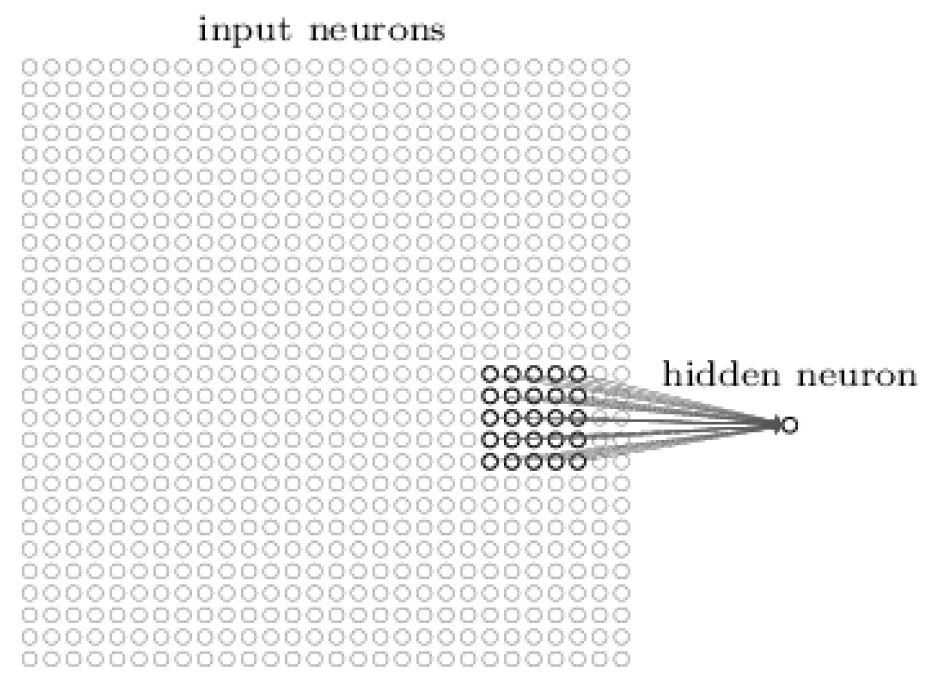
\includegraphics[width=0.7\textwidth]{Images/receptive_field}
		\caption{Implementation of a $5x5$ receptive field in a \acs{CNN}}\label{fig:receptive_field}
	\end{figure}
	
	\item[3D volumes of neurons] Neurons inside a \acs{CNN} are arranged in 3 dimensions: width, height and depth. Neurons inside a layer are only connected to a small region of the layer before it, called a receptive field. Figure \ref{fig:receptive_field}, for instance, shows a $5x5$ receptive field from the input neurons to the first hidden layer, with a $28x28$ input.
	
	\item[Local connectivity] Following the concept of receptive field, \acsp{CNN} exploit spatially local correlation by enforcing a local connectivity pattern between neurons of adjacent layers. The architecture, thus, ensures that every \textbf{filter} (\ie weight patch) learnt produces the strongest response to a spatially local input pattern. Stacking many of such layers leads to non-linear filters that become increasingly "global" (\ie responsive to a larger region of input space). This allows the network to first create good representations of small parts of the input, then assemble representations of larger areas from them.  Distinct types of layers, both locally and completely connected, are stacked to form the \acs{CNN} architecture.
	
	\item[Shared weights] In \acsp{CNN}, each filter is replicated across the entire visual field. These replicated units share the same parameterization (weight vector and bias) and produce a feature map. This means that all the neurons in a given convolutional layer detect exactly the same features. Replicating units in this way allows for features to be detected regardless of their position in the visual field, thus constituting the property of translation invariance.
	
\end{description}

Together, these properties allow convolutional neural networks to achieve better generalization performances in vision problems. Moreover, the weight sharing helps by dramatically reducing the number of free parameters the network has to learn, thus lowering the memory requirements for running the network. Decreasing the memory footprint allows the training of larger and more powerful networks.

\section{The convolution operation}

In its most general form, convolution is an operation on two functions of a real-valued argument. It produces a third function, that is typically viewed as a modified version of one of the original functions, giving the integral of the point-wise multiplication of the two functions as a function of the amount that one of the original functions is translated. It is typically
denoted with an asterisk and it is defined as:

\begin{figure}[t]
	\centering
	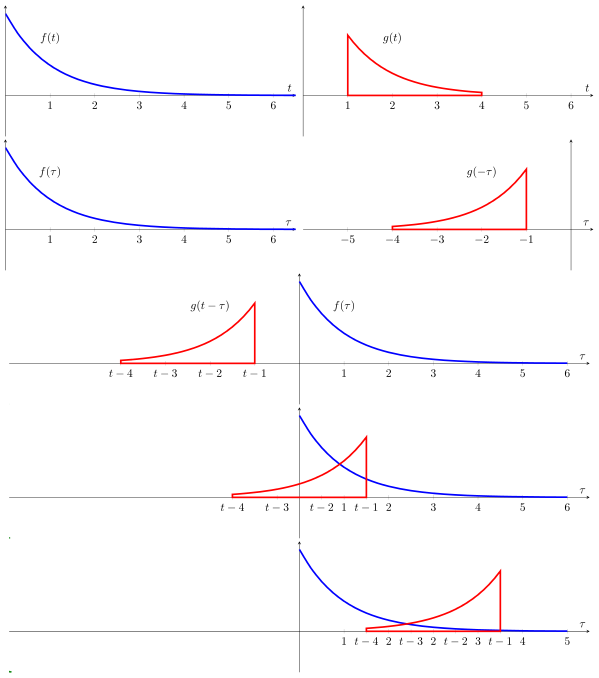
\includegraphics[width=0.7\textwidth]{Images/convolution}
	\caption{Visual explanation of the convolution operation}\label{fig:convolution}
\end{figure}

\begin{equation} \notag
	s(t) = (f * g)(t) = \int_{-\infty}^{\infty}f(\tau)g(t-\tau)\,d\tau
\end{equation}

The convolution formula can be described as a weighted average of the function $f(\tau)$ at moment $t$ where the weighting is given by $g(-\tau)$ simply shifted by amount $t$. As $t$ changes, the weighting function emphasizes different parts of the input function. The output is sometimes referred to as \textbf{feature} or  \textbf{activation map}.

Figure \ref{fig:convolution} shows a visual explanation of the operation. Wherever the two functions intersect, the integral of their product is found. In other words, it computes a sliding, \ie  a weighted-sum of function $f(\tau)$, where the weighting function is $g(-\tau)$.

If we now assume that $f$ and $g$ are defined only on integer $t$, we
can define the discrete convolution as:

\begin{equation} \notag
	s(t) = (f * g)(t) = \sum_{-\infty}^{\infty}f(\tau)g(t-\tau)
\end{equation}

In convolutional networks terminology, the first argument of the convolution is often referred to as input and the second as \textbf{kernel} or \textbf{filter}. In machine learning applications, the input is usually a multidimensional array (\ie a tensor) of data and the kernel is usually a multidimensional array of parameters that are adapted by the learning algorithm.

\begin{figure}[ht]
	\centering
	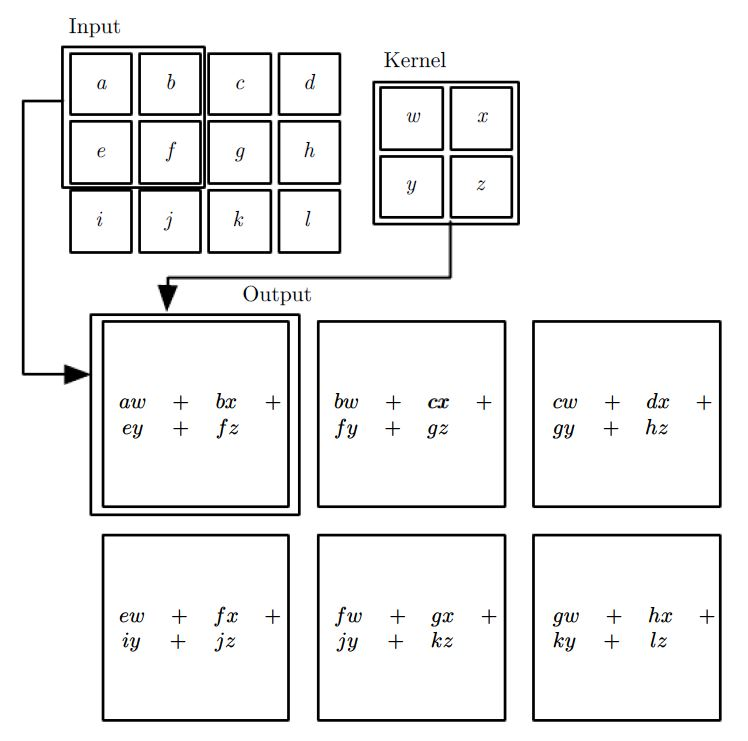
\includegraphics[width=0.7\textwidth]{Images/convolution_example}
	\caption{Example of convolution without kernel-flipping, as reported in [\cite{Goodfellow-et-al-2016}]}\label{fig:convolution_example}
\end{figure}

Figure \ref{fig:convolution_example} shows an example of convolution (without kernel flipping) applied to a 2D tensor. In this case, the output is restricted to only positions where the kernel lies entirely within the image.

\section{Architecture}

A \acs{CNN} architecture is formed by a stack of distinct layers that transform the input volume into an output volume through a differentiable function. A few distinct types of layers are commonly used and they are described below.

\subsection{Convolutional layer}

The \textbf{convolutional layer} is the core building block of a \acs{CNN}. The layer's parameters consist of a set of learnable filters (or kernels), which have a small receptive field, but extend through the full depth of the input volume. During the forward pass, each filter is convolved across the dimensions of the input volume, computing the dot product between the entries of the filter and the input, producing a feature map of that filter.

The amount of units by which the filter shifts is called \textbf{stride} and it controls how the filter convolves around the input volume.

As a result of this process, the network learns filters that activate when they detect some specific type of features in a given spatial position in the input.

\begin{figure}
	\centering
	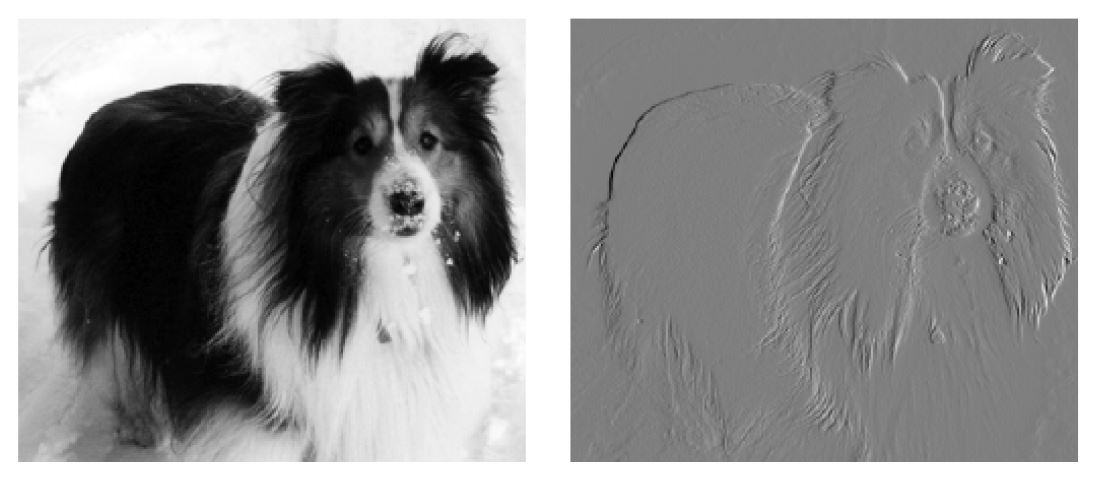
\includegraphics[width=0.7\textwidth]{Images/filter_application}
	\caption{Application of a filter for edge detection (Source: [\cite{Goodfellow-et-al-2016}])}\label{fig:filter_application}
\end{figure}

It is evident that different filters will produce different feature maps for the same input. Figure \ref{fig:filter_application} shows the result of the application of a filter for edge detection to a given image. The image on the right was formed by taking each pixel in the original image and subtracting the value of its neighboring pixel on the left. This shows the strength of all of the vertically oriented edges in the input image, which can be a useful operation for object detection.

Stacking the activation maps for all filters along the depth dimension forms the full output volume of the convolution layer. Every entry in the output volume can thus also be interpreted as an output of a neuron that looks at a small region in the input and shares parameters with neurons in the same activation map.

In fact, in order to recognize an image, we'll need more than one filter. For this reason, the output of a full convolutional layer will be a set of feature maps with a structure similar to the one in figure \ref{fig:feature_maps}.

\begin{figure}[ht]
	\centering
	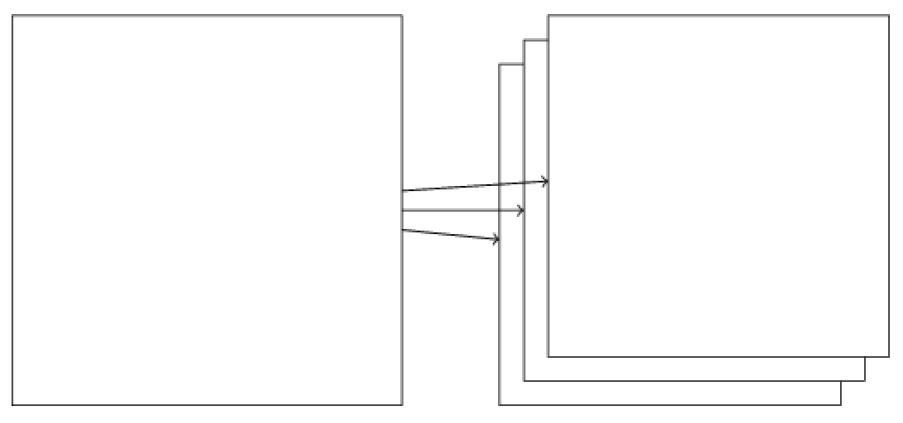
\includegraphics[width=0.7\textwidth]{Images/feature_maps}
	\caption{Application of three filters to a given input producing three different feature maps}\label{fig:feature_maps}
\end{figure}

\begin{figure}[ht]
	\centering
	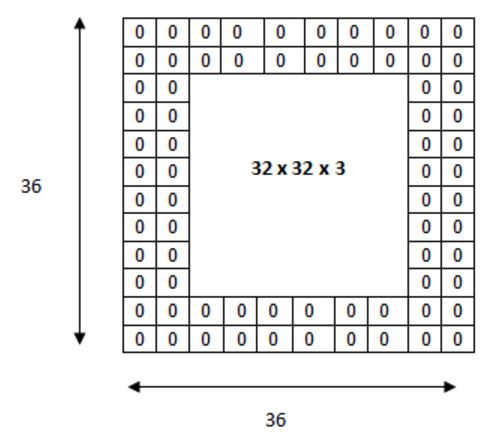
\includegraphics[width=0.7\textwidth]{Images/zero_padding}
	\caption{Zero padding of two applied to a $32x32x3$ picture}\label{fig:zero_padding}
\end{figure}

Sometimes it is convenient to have an output of the same size of the input. In this case it is necessary to add some additional pixels to the input image; this operation is called \textbf{padding}. For instance, a zero padding like the one in figure \ref{fig:zero_padding} pads the input volume with zeros all around the border.
The size of this zero-padding is an optional hyperparameter. Zero padding, in particular, provides control of the output volume spatial size.

In general, the formula for calculating the output size for any given convolutional layer is:

\begin{equation} \notag
	O=\frac{W-K+2P}{S}+1
\end{equation}
where O is the output height/length, W is the input height/length, K is the filter size, P is the padding, and S is the stride. If this number is not an integer, then the strides are set incorrectly and the neurons cannot be tiled to fit across the input volume in a symmetric way.

Setting the padding to
\begin{equation} \notag
	P=\frac{K-1}{2}
\end{equation}
when the stride is $S=1$ ensures that the input volume and output volume will have the same size spatially.

\subsection{ReLU layer}

After a convolutional layer, it is convention to apply a non-linear layer (or activation layer) immediately afterward. The purpose of this layer is to introduce non-linearity to a system that basically has just been computing linear operations during the convolution operation (just element wise multiplications and summations). This is a layer of neurons which applies the non-saturating activation function:
\begin{equation} \notag
	f(x)=\max(0,x)
\end{equation}

\begin{figure}[!ht]
	\centering
	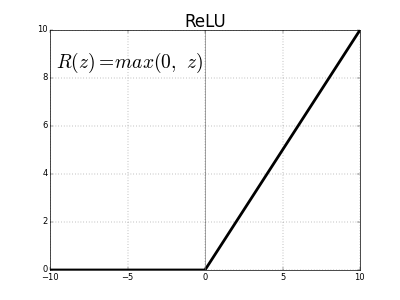
\includegraphics[width=0.5\textwidth]{Images/relu_function}
	\caption{\ac{ReLU} function}\label{fig:relu_function}
\end{figure}

This increases the non-linear properties of the decision function and of the overall network without affecting the receptive fields of the convolution layer. The output of this layer is known as \textbf{rectified feature map}.

In the past, non-linear functions like $tanh$ and sigmoid were used, but researchers found out that \ac{ReLU} layers work far better because the network is able to train a lot faster (because of the computational efficiency) without significant reductions in the accuracy [\cite{icml2010_NairH10}]. Using a \ac{ReLU} function also helps to alleviate the vanishing gradient problem, which is the issue where the lower layers of the network train very slowly because the gradient decreases exponentially through the layers.

\begin{figure}
	\centering
	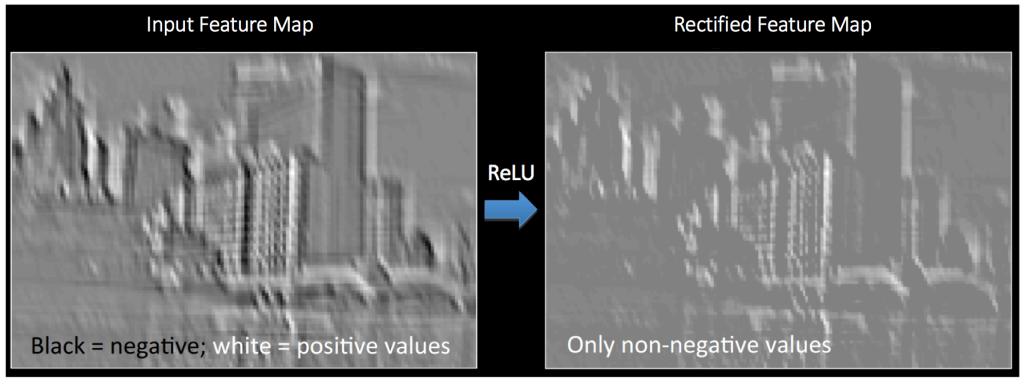
\includegraphics[width=0.7\textwidth]{Images/relu}
	\caption{\ac{ReLU} operation. Source \url{http://mlss.tuebingen.mpg.de/2015/slides/fergus/Fergus_1.pdf}}\label{fig:relu}
\end{figure}

The ReLU layer applies the function $f(x) = max(0, x)$ to all of the values in the input volume. In basic terms, this layer just changes all the negative activations to 0. Figure \ref{fig:relu} shows the input of a \ac{ReLU} layer and the resulting output.

\subsection{Pooling layer}

Another important concept of \acsp{CNN} is \textbf{pooling}, which is a form of non-linear down-sampling. There are several non-linear functions to implement pooling among which \textbf{max pooling} is the most common. It partitions the input image into a set of non-overlapping regions and, for each of them, outputs the maximum value.

The intuition is that once a feature has been found, its exact location isn't as important as its rough location relative to other features. The function of the pooling layer is to progressively reduce the spatial size of the representation to reduce the amount of parameters and computation in the network, and hence to control overfitting, too. It is common to periodically insert a pooling layer in-between successive convolutional/\acs{ReLU} layers in a \acs{CNN} architecture.

The pooling operation also provides a form of translation invariance. This is very powerful since we can detect objects in an image no matter where and how they are located.

\begin{figure}[b]
	\centering
	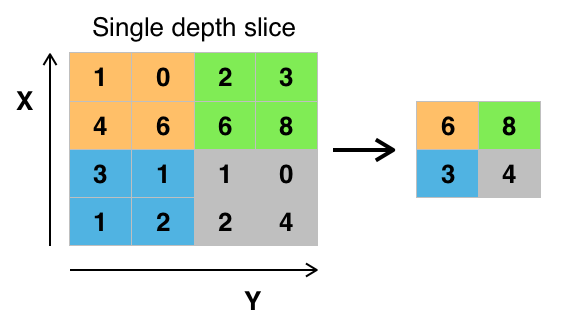
\includegraphics[width=0.7\textwidth]{Images/max_pooling}
	\caption{Max pooling with a $2x2$ filter and stride $S=2$}\label{fig:max_pooling}
\end{figure}

The pooling layer operates independently on every depth slice of the input and resizes it spatially. This operation is also known as \textbf{subsampling} or \textbf{downsampling}. The most common form is a pooling layer with filters of size $2x2$ applied with a stride of 2. Every operation would in this case be taking a max over 4 numbers. Figure \ref{fig:max_pooling} shows an example of this operation.

In addition to max pooling, the pooling units can also perform other functions, such as average pooling and even L2-norm pooling. Average pooling was often used historically but has recently fallen out of favor compared to the max pooling operation, which has been found to work better in practice, as reported in [\cite{Scherer:2010}].

Due to the aggressive reduction in the size of the representation (which is helpful only for smaller datasets to control overfitting), the current trend in the literature is towards using smaller filters [\cite{DBLP:journals/corr/Graham14a}] or completely discarding the pooling layer [\cite{DBLP:journals/corr/SpringenbergDBR14}].

Obviously, the pooling operation is applied separately to each feature map.

\subsection{Fully connected layer}

Finally, after several convolutional/\ac{ReLU} and max pooling layers, the high-level reasoning in the neural network is done via \textbf{fully connected layers}. Neurons in a fully connected layer have full connections with all the activations in the previous layer, as in traditional \acsp{MLP}. Their activations can hence be computed with a matrix multiplication followed by a bias offset.

The output from the convolutional and pooling layers represent high-level features of the input image. The purpose of the fully connected layer is usually to use these features for classifying the input into various classes based on the training dataset. For instance, the image classification task aims to put a given image into a precise category.

Apart from classification, adding a fully-connected layer is also a cheap way of learning combinations of these features. Most of the features from convolutional and pooling layers may be good for the classification task, but combinations of those features might be even better.

\subsection{Dropout layer}

\textbf{Dropout layers} have a very specific function in neural networks: they reduce overfitting. The problem of overfitting is very important in machine learning. It happens when after training, the weights of the network are so tuned to the training examples given that the network doesn't perform well when given new examples (\ie it doesn't generalize).

The idea of dropout is simplistic in nature. This layer "drops out" a random set of activations in that layer by setting them to zero in the forward pass. At each training epoch, individual nodes are either "dropped out" from the net with probability $1-p$ or kept with probability $p$, where $p$ is a user-defined parameter, so that a reduced network is left. The removed nodes are then reinserted into the network with their original weights.

This pruning, in a way, forces the network to be redundant; the network should be able to provide the right classification or output for a specific example even if some of the activations are dropped out.

This makes sure that the network isn’t getting too "fitted" to the training data and, thus, helps alleviating the overfitting problem. An important note is that this layer is only used during training.

The method also significantly improves the speed of training. This makes model combination practical, even for deep neural networks. The technique seems to reduce the complex, tightly fitted interactions between nodes, leading them to learn more robust features which better generalize to new data. Dropout has been shown to improve the performance of neural networks on tasks in vision, speech recognition, document classification, and computational biology.

An interesting analysis of the use of dropout in order to manage overfitting can be found in [\cite{Srivastava:2014:DSW:2627435.2670313}]

\subsection{Loss layer}

Finally, a loss layer specifies how the network training penalizes the deviation between the predicted and true labels. This is normally the last layer in the network. Various loss functions appropriate for different tasks may be used there. 

\textbf{Softmax loss} is used for predicting a class of K different classes (\ie the digit represented by an image from the MNIST dataset of handwritten digits, see chapter \ref{ch:basic_tf_model} for further details).

The function
\begin{equation} \notag
	f_j(z)=\frac{e^{z_j}}{\sum_{k}e^{z_k}}
\end{equation}
is called the softmax function: it takes a vector of arbitrary real-valued scores and squashes it to a vector of values between zero and one that sum to one.

Moreover, sigmoid cross-entropy loss is used for predicting K independent probability values in $[0,1]$. Euclidean loss is used for regressing to real-valued labels in $[-\infty ,\infty ]$.

\bigskip

These layers are the basic building blocks of any \acs{CNN}. They can be stacked in order to produce complex architectures. The number of layers depends on the addressed task and on the complexity of the input. A typical convolutional architecture is composed by one or more sets of convolutional, \acs{ReLU} and pooling layers and ends with a fully connected, a dropout and a loss layer. Again, the loss function to use depends on the task to be solved.

\begin{figure}
	\centering
	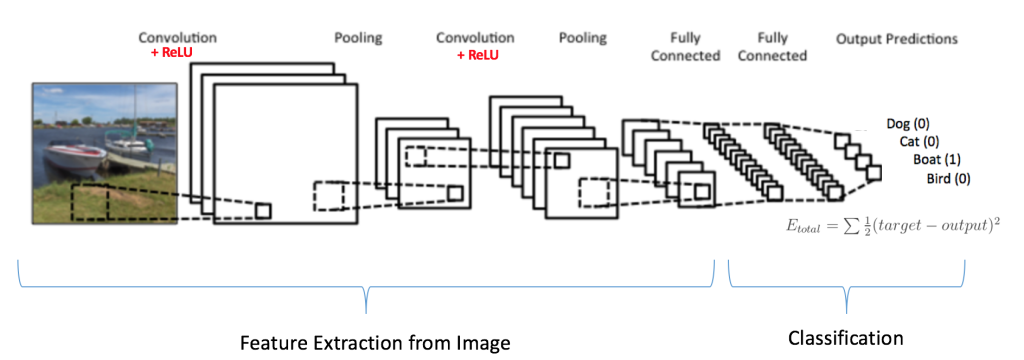
\includegraphics[width=0.9\textwidth]{Images/conv_architecture}
	\caption{Convolutional neural network for the classification of an image}\label{fig:conv_architecture}
\end{figure}

Figure \ref{fig:conv_architecture} shows an example of architechture for image recognition with two convolutional layers and two pooling layers.

Many different architectures have been proposed. Among them, LeNet [\cite{lecun-98}] was one of the very first convolutional neural networks, for the recognition of handwritten digits, which helped propel the field of deep learning. In 2012, Alex Krizhevsky and others released AlexNet [\cite{krizhevsky2012imagenet}] which was a deeper and much wider version of the LeNet and won by a large margin the difficult \href{http://image-net.org/challenges/LSVRC/2012/index}{ImageNet Large Scale Visual Recognition Challenge (ILSVRC)} in 2012. The ILSVRC 2014 winner was GoogleNet, a convolutional network from [\cite{DBLP:journals/corr/SzegedyLJSRAEVR14}] from Google. Its main contribution was the development of an Inception Module that dramatically reduced the number of parameters in the network. In 2016 GoogleNet (now called Inception) is at its third release.

\section{Hyperparameters}


\acp{CNN} use more hyperparameters than a standard \ac{MLP}. While the usual rules for learning rates and regularization constants still apply, the following should be kept in mind when optimising a convolutional network [\cite{conv_wiki}].

\begin{description}
	
	\item[Number of filters] Since feature map size decreases with depth, layers near the input layer will tend to have fewer filters while layers higher up can have more. To equalize computation at each layer, the product of the number of features and the number of pixel positions is typically picked to be roughly constant across the layers. Preserving the information about the input would require keeping the total number of activations (number of feature maps times number of pixel positions) to be non-decreasing from one layer to the next.
	The number of feature maps directly controls capacity and depends on the number of available examples and on the complexity of the task.
	
	\item[Filter shape and size] Common filter shapes vary greatly in the literature, and are usually chosen based on the dataset. The challenge is, thus, to find the right level of granularity so as to create abstractions at the proper scale, given a particular dataset.
	
	\item[Max Pooling Shape] Typical values are $2x2$. Very large input volumes may warrant $4x4$ pooling in the first layers. However, choosing larger shapes will dramatically reduce the dimension of the signal, and may result in discarding too much information. Often, non-overlapping pooling windows perform best, as shown in [\cite{Scherer:2010}].
	
	\item[Amount of examples] For many applications, only a small amount of training data is available. Convolutional neural networks usually require a large amount of training data in order to avoid overfitting. A common technique is to train the network on a larger data set from a related domain. Once the network parameters have converged an additional training step is performed using the in-domain data to fine-tune the network weights. This allows convolutional networks to be successfully applied to problems with small training sets.
	
\end{description}

\section{Applications}

We conclude this chapter with some examples of application on \acp{CNN} in real-world domains. These kind of networks can be used with success to solve many different task, but, as said before, they work well with data with a grid-like topology.

\subsection{Image recognition}

Convolutional neural networks are often used in image recognition systems. They have achieved an error rate of 0.23 percent on the MNIST database, which as of February 2012 is the lowest achieved on the database [\cite{6248110}]. When applied to facial recognition, they were able to contribute to a large decrease in error rate [\cite{554195}].

The \href{http://www.image-net.org/challenges/LSVRC/}{ImageNet Large Scale Visual Recognition Challenge} is a benchmark in object classification and detection, with millions of images and hundreds of object classes. In the ILSVRC 2014, almost every highly ranked team used a \ac{CNN} as basic framework. The winner GoogLeNet [\cite{DBLP:journals/corr/SzegedyLJSRAEVR14}] (the foundation of Google DeepDream) increased the mean average precision of object detection to 0.439329, and reduced classification error to 0.06656, the best result to date. Its network applied more than 30 layers.

The performance of convolutional neural networks on the ImageNet tests is now close to that of humans. In 2015 a many-layered CNN demonstrated the ability to spot faces from a wide range of angles, including upside down, even when partially occluded with competitive performance [\cite{DBLP:journals/corr/FarfadeSL15}].

\subsection{Video analysis}

Compared to image data domains, there is relatively little work on applying \acp{CNN} to video classification. Video is more complex than images since it has another (temporal) dimension. However, some extensions of convolutional neural networks into the video domain have been explored. One approach is to treat space and time as equivalent dimensions of the input and perform convolutions in both time and space [\cite{6165309}].

\subsection{Natural language processing}

Convolutional neural networks have also seen use in the field of natural language processing. \ac{CNN} models have subsequently been shown to be effective for various \acs{NLP} problems and have achieved excellent results in semantic parsing, search query retrieval, sentence modeling, classification, prediction, and other traditional \acs{NLP} tasks.

\subsection{Drug discovery}

Convolutional neural networks have been used in drug discovery. Predicting the interaction between molecules and biological proteins can be used to identify potential treatments that are more likely to be effective and safe.

In 2015, Atomwise introduced AtomNet, the first deep learning neural network for structure-based rational drug design. [\cite{DBLP:journals/corr/WallachDH15}]
Subsequently, AtomNet was used to predict novel candidate biomolecules for several disease targets, most notably treatments for the Ebola virus and multiple sclerosis.

\subsection{Playing Go}

Convolutional neural networks have been used in computer Go. In December 2014, Christopher Clark and Amos Storkey published a paper ([\cite{DBLP:journals/corr/ClarkS14}]) showing a convolutional network trained by supervised learning from a database of human professional games could outperform GNU Go and win some games against Monte Carlo tree search Fuego 1.1 in a fraction of the time it took Fuego to play.

Shortly after it was announced that a large 12-layer convolutional neural network had correctly predicted the professional move in 55\% of positions, equalling the accuracy of a 6 dan human player.

Finally, a couple of \acp{CNN} for choosing moves and evaluating positions were used by \href{https://deepmind.com/research/alphago/}{AlphaGo}, Google Deepmind's program that was the first to beat a professional human player.